\chapter{Documento de Arquitectura de Software}\label{apendice.C}
\section{Introducción}
Este documento brinda una vista general de alto nivel sobre cómo será el desarrollo del sistema JigsawCoding. Se resumirá las tecnologías con las cuales se implementará el sistema así como también se proporcionará una descripción de alto nivel de la arquitectura del sistema.
\subsection{Propósito}
El presente documento de arquitectura de software tiene como finalidad describir el sistema web Jigsaw Coding desde diferentes vistas arquitectónicas, las cuales serán de gran utilidad para el desarrollo de dicho sistema.
\subsection{Alcance} Este documento arquitectónico aplica para describir las características arquitectónicas del sistema web JigsawCoding, las tecnologías que serán usadas en su desarrollo y las principales funcionalidades del sistema.
\subsection{Definiciones, acrónimos y abreviaturas}
En esta sección se provee las definiciones, acrónimos y abreviaturas de términos utilizados en el presente documento a fin de brindar al lector una mejor comprensión del contenido. 
\clearpage
\begin{longtable}{|c|L{8cm}|}
    \hline
  SJC & Sistema Jigsaw Coding \\ \hline
  UML & Unified Modeling Language: Lenguaje Unificado de Modelamiento \\ \hline
  CRUD & Create - Read - Update - Delete \\ \hline
  JSON & JavaScript Object Notation: Es un formato ligero para el intercambio de datos \\ \hline
  XML & eXtensible Markup Language: Es un lenguaje de marcas utilizado para almacenar datos en forma legible. \\ \hline
  \emph{sbt} & Herramienta de construcción interactiva \url{http://www.scala-sbt.org} \\ \hline
\end{longtable}
\subsection{Metas arquitectónicas y restricciones}

\subsubsection{Plataforma técnica}
\begin{itemize}
	\item El sistema jigsaw coding debe ser desplegado en un servidor web que soporte el framework Play. Para ello se ha decidido usar la plataforma Heroku.
	\item La base de datos del sistema también estará alojada en la plataforma Heroku y será una base de datos Postgres.
\end{itemize}

\subsubsection{Persistencia}
La persistencia se logrará utilizando una base de datos relacional y el mapeo de entidades a tablas estará a cargo del ORM Ebean que por defecto viene incluído en el framework Play.

\subsubsection{Seguridad}
La seguridad del sistema está basada en perfiles. La aplicación contendrá los siguientes puntos:

\begin{itemize}
	\item Autenticación: Cada usuario deberá identificarse con su email y password para poder acceder al sistema.
	\item Autorización: El sistema cuenta con dos perfiles(Docente y Alumno) y dependiendo de ello, el usuario podrá ingresar a diferentes partes del sistema.
\end{itemize}

\subsubsection{Confiabilidad - Disponibilidad}
Para el sistema se busca tener una confiabilidad y disponibilidad de casi un 100\%. El sistema debe estar disponible las 24 horas del día, 7 días a la semana.

\section{Representación arquitectónica}
El sistema web JigsawCoding, será implementado usando una arquitectura Modelo - Vista - Controlador, la misma que está definida en el framework Play de Java.
\subsection{PlayFramework 2.2.4}
Play es framework open source de Java y Scala que integra componentes y APIs necesarios para el desarrollo moderno de aplicaciones web. Play sigue el patrón de arquitectura Modelo - Vista - Controlador y uno de sus objetivos es optimizar la productividad del desarrollador a través del uso de configuraciones estandarizadas, recompilación automática del código fuente y la visualización de errores directamente en el navegador.\\

A pesar que las aplicaciones de Play están diseñadas para correr en servidores web basados en Jboos Netty, también pueden ser deployadas como archivos WAR para ser distribuidos en la mayoría de servidores de aplicaciones Java EE como Apache Tomcat o GlassFish.

\subsubsection{Componentes y Características de Play}
\begin{itemize}
  \item JBoss Netty para el servidor web.
  \item Ebean como ORM para Java.
  \item Scala para el motor de plantillas.
  \item Recompilación de código automática.
  \item \emph{sbt} para la administración de dependencias.
  \item CRUD: un módulo para simplificar la edición de objetos.
  \item Secure: un módulo para establecer simples autenticaciones de usuarios.
  \item Parsers de JSON y XML.
%  \item Una capa de persistencia basada en JPA
\end{itemize}
\clearpage
\section{Vista Lógica}
\begin{figure}[!h]
	\centering
	% Requires \usepackage{graphicx}
	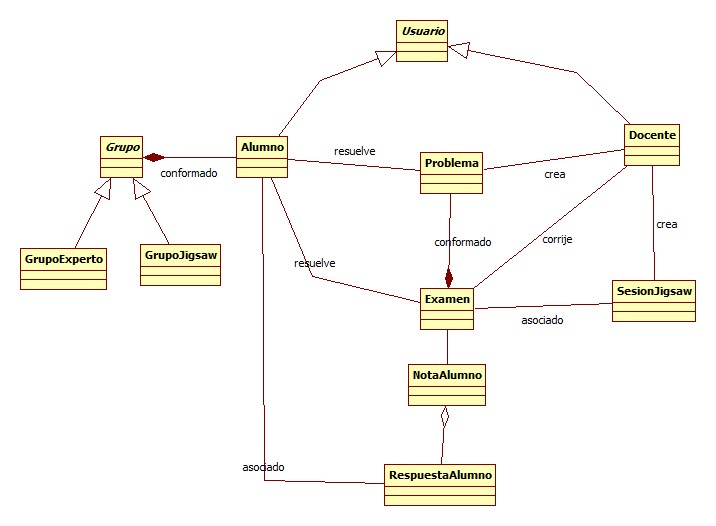
\includegraphics[scale=0.6]{figuras/sad/diagrama_de_clases.jpg}\\
	\caption{Diagrama de Clases}\label{fig:diagrama_de_clases}
\end{figure}
Tal como se puede observar en el Diagrama de clases de la figura \ref{fig:diagrama_de_clases}:\\

El Sistema Jigsaw Coding permite el acceso a Usuario lo cuales pueden ser de dos tipos: Docente o Alumno. El docente puede crear problemas y además es el encargado de crear las sesiones jigsaw. El docente también es quien crea los examenes, los cuales están conformados por un conjunto de problemas y cada examen es resuelto por los alumnos, quienes para tal objetivo, deben resolver los problemas que componen cada examen. Por otro lado, los alumnos también resuelven problemas cada vez que se encuentran dentro de un grupo de expertos o un grupo jigsaw. Naturalmente, los examenes son evaluados por el docente y éste les asigna una nota a cada una de las respuestas que los alumnos envía al terminar su examen.
\clearpage
\section{Vista de Desarrollo}
La vista de despliegue muestra el sistema desde la perspectiva del programador y se ocupa de la gestión del software a implementar. Esto es, en esta vista se describe cómo estará dividido el sistema JigsaCoding en paquetes y las dependencias que habrá entre ellos.
\begin{figure}[!h]
  \centering
  % Requires \usepackage{graphicx}
  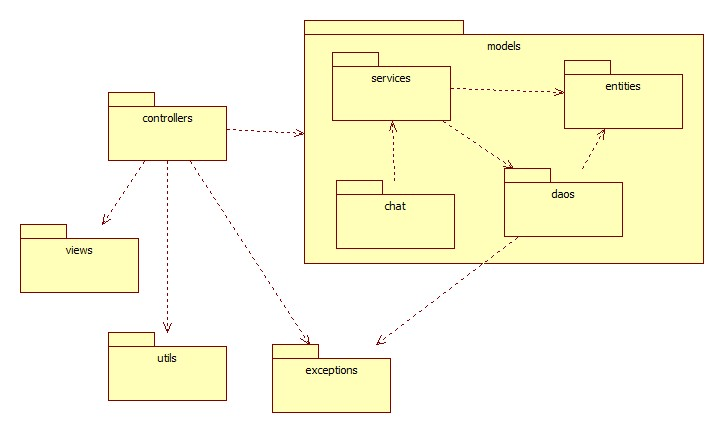
\includegraphics[scale=0.6]{figuras/sad/diagrama_de_paquetes.jpg}\\
  \caption{Diagrama de Paquetes}\label{fig:diagrama_de_paquetes}
\end{figure}
\begin{itemize}
  \item \textbf{controllers}\\Este paquete contiene todas las clases Controladores que sirven para gestionar el ruteo de páginas del sistema.
  \item \textbf{models}\\En este paquete se encuentran las clases de Servicios, Entidades y Acceso a Datos que son requeridas para el sistema.
  \item \textbf{views}\\Este paquete contiene todas las plantillas (\emph{*.scala.html}) que permitirán renderizar las páginas web del sistema.
\end{itemize}
\clearpage
\section{Vista Física}
\begin{figure}[!h]
  \centering
  % Requires \usepackage{graphicx}
  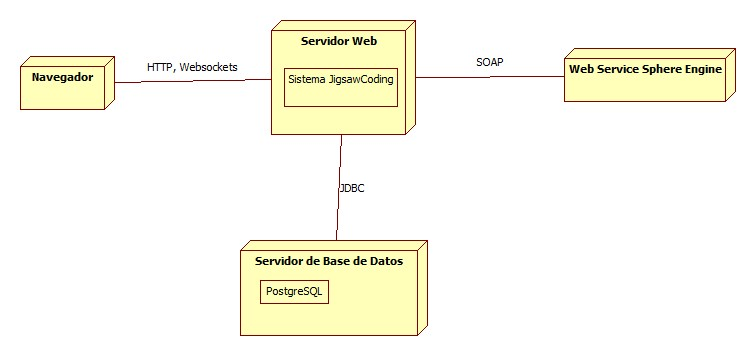
\includegraphics[scale=0.5]{figuras/sad/diagrama_de_despliegue.jpg}\\
  \caption{Diagrama de Despliegue}\label{fig:diagrama_de_despliegue}
\end{figure}
\begin{itemize}
  \item \texttt{Navegador}\\Es la interfaz que permitirá visualizar el contenido de las páginas web del Sistema Jigsaw Coding. 
  \item \texttt{Servidor Web}\\Es el responsable de gestionar todas las peticiones HTTP provenientes de los navegadores web y de enviar las respuestas con los datos solicitados por los mismos. La comunicación entre el servidor web y el navegador se realiza vía los protocolos HTTP y Websockets, este último, es usado para el envío de mensajes entres los usuarios via chat.
  \item \texttt{Servidor de Base de Datos}\\Es el lugar donde estará almacenada la información del Sistema Web JigsawCoding.
  \item \texttt{Web Service Sphere Engine}\\Es un servicio web que servirá para compilar y ejecutar el código fuente desarrollado por los usuarios del sistema.
\end{itemize}
%\clearpage
\section{Vista de Escenarios}
La vista de escenarios o vista de casos de uso es la encargada de presentar la percepción que tiene el usuario sobre las distintas funcionalidades del sistema.
\begin{landscape}

\begin{figure}[!h]
  \centering
  % Requires \usepackage{graphicx}
  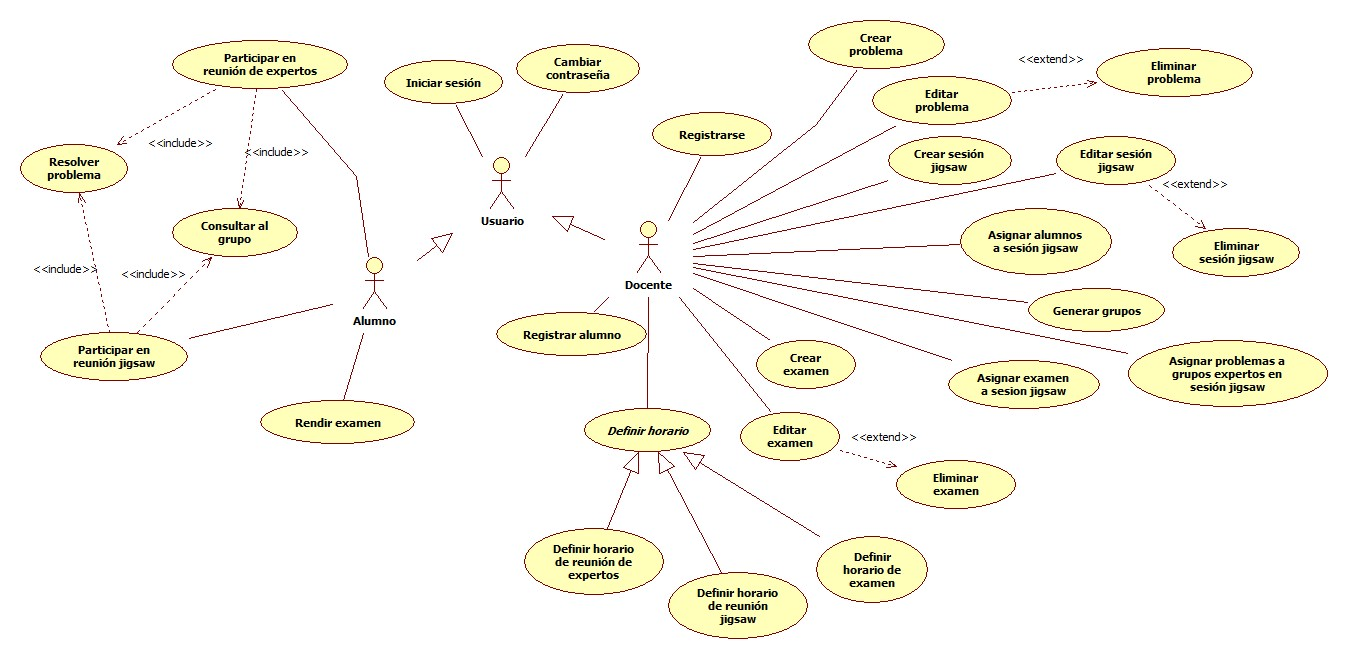
\includegraphics[scale=0.45]{figuras/casosdeuso/casos_de_uso.jpg}\\
  \caption[Casos de uso]{Diagrama de casos de uso para el sistema JigsawCoding}
  \label{fig:casos_de_uso}
\end{figure}
\end{landscape}

\subsection{Catálogo de actores}
En la siguiente figura se puede ver los actores que participan en el Sistema Jigsaw Coding y en la Tabla \ref{tab:das_actores} se encuentra una breve descripción de cada uno de ellos.
\begin{figure}
	\centering
	% Requires \usepackage{graphicx}
	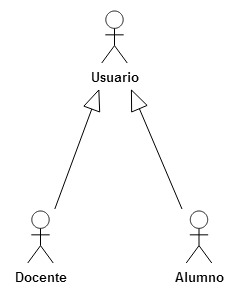
\includegraphics[scale=0.6]{figuras/casosdeuso/actores.jpg}\\
	\caption[Diagrama de actores]{Diagrama de actores}
	\label{fig:das_actores}
\end{figure}

\begin{longtable}{|L{3cm}|L{7cm}|}
	\caption{Actores}
	\label{tab:das_actores}\\
	\hline
	ACTOR & DESCRIPCIÓN \\
	\hline
	Usuario & Persona que usará el sistema web de tiempo real para el aprendizaje colaborativo.\\
	\hline
	Docente & Es la persona responsable de crear y dirigir las sesiones de clase que serán aplicadas a los alumnos. Además, el docente es el responsable de las evaluaciones que rendirán los alumnos una vez terminada cada sesión de clase.\\
	\hline
	Alumno & Es la persona que será instruida en temas de algoritmos y programación a través de cada sesión diseñada por el docente.\\
	\hline
\end{longtable}

\subsubsection{Casos de uso}
En la tabla siguiente se presenta la descripción breve de los casos de uso obtenidos para el Sistema Jigsaw Coding, estos son especificados de una manera más detallada en el anexo \ref{apendice.A}\\
\clearpage
\begin{longtable}{|L{4cm}|L{9cm}|}
	\caption{Casos de uso}
	\label{tab:das_casosdeuso}\\
	\hline
	CASO DE USO & DESCRIPCIÓN \\
	\hline
	Registrar alumno & Este caso de uso define los pasos que el usuario con perfil docente debe seguir para poder registrar un alumno en el sistema.\\
	\hline
	Crear Problema & El caso de uso crear problema detalla la interacción entre el sistema y el usuario docente cada vez que éste necesite crear un problema o ejercicio en el sistema.\\
	\hline
	Crear sesión jigsaw & Este caso de uso describe la secuencia de pasos que se debe seguir para poder crear una sesión de clase basada en la técnica de aprendizaje colaborativo jigsaw.\\
	\hline
	Asignar alumno sesión jigsaw & Las sesiones jigsaw necesitan tener alumnos y ese es el objetivo que tine este caso de uso.\\
	\hline
	Generar grupos & Mediante este caso de uso, el Sistema Jigsaw Coding realiza la creación de grupos expertos y grupos jigsaw y a cada uno de ellos les asigna alumnos de forma aleatoria.\\
	\hline
	Asignar problemas a grupos expertos & En este caso de uso se describe cómo el usuario docente puede asignar un problema a cada grupo experto generado por el sistema para una determinada sesión jigsaw.\\
	\hline
	Crear examen & El caso de uso detalla la manera en la que el usuario docente puede crear un examen, el mismo que será usado para la fase de evaluación de la sesión jigsaw.\\
	\hline
	Definir horario de reunión de expertos & Este caso de uso sirve para establecer la fecha y hora de inicio de la reunión de expertos así como su respectiva duración.\\
	\hline
	Definir horario de reunión jigsaw & Este caso de uso sirve para establecer la fecha y hora de inicio de la reunión jigsaw así como su respectiva duración.\\
	\hline
	Definir horario de examen & Este caso de uso sirve para establecer el intervalo de tiempo en el cual se puede acceder a examen así como también su respectiva duración.\\
	\hline
	Unirse a reunión de expertos & Este caso de uso le sirve al usuario alumno para poder ingresar a la reunión de expertos y desarrollar el problema asignado junto con los demás integrantes del grupo.\\
	\hline
	Unirse a reunión jigsaw & Este caso de uso le sirve al usuario alumno para poder ingresar a la reunión jigsaw y desarrollar los respectivos problemas junto con los demás integrantes del grupo. \\
	\hline
	Resolver problema & El caso de uso describe la interacción entre el usuario alumno y el sistema cada vez que se requiere resolver un problema asignado por el usuario docente.\\
	\hline
	Rendir examen & El caso de uso le permite al usuario alumno acceder al examen y visualizar cada una de las preguntas que debe resolver.\\
	\hline
	Consultar al grupo & Este caso de uso describe la manera en la que un usuario alumno puede consultar con los demás integrantes de su grupo experto o grupo jigsaw.\\
	\hline
\end{longtable}

\clearpage
\section{Vista de Datos}
\begin{figure}[!h]
  \centering
  % Requires \usepackage{graphicx}
  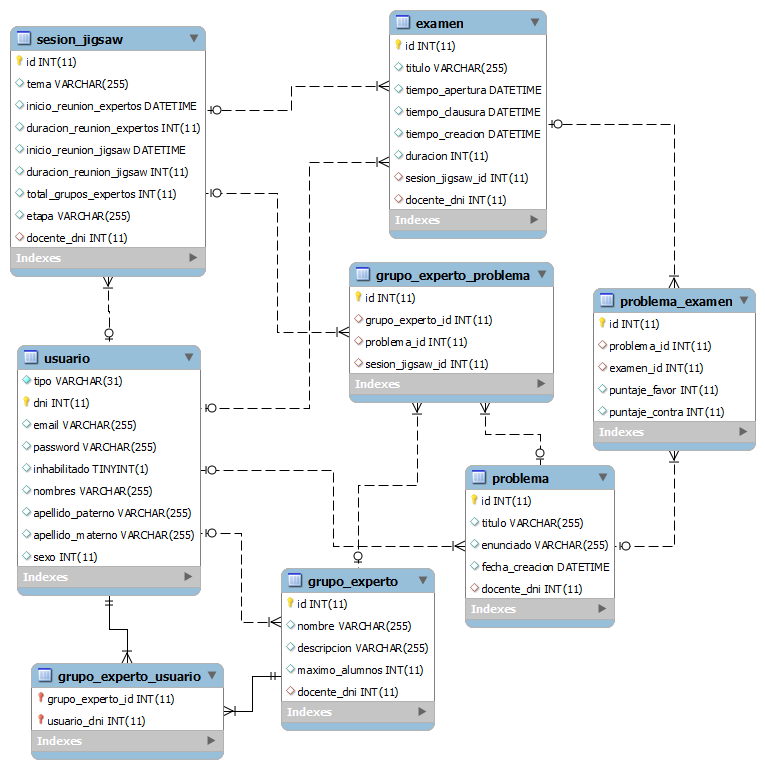
\includegraphics[scale=0.45]{figuras/sad/modelo_de_datos.png}\\
  \caption[Modelo de datos]{Modelo de base de datos del sistema JigsawCoding}\label{fig:modelo_de_datos}
\end{figure}
\subsection{PostgreSQL}
El desarrollo del sistema JigsawCoding se hará usando como motor de base de datos a PostgreSQL en su versión 9.3. 
\subsection{Diccionario de datos}
A continuación, el la tabla \ref{tab:das_diccionario_datos} se muestra la descripción de las tablas que conforman el modelo de datos del sistema Jigsaw Coding mostrado en la figura \ref{fig:modelo_de_datos}.
\begin{longtable}{|L{4cm}|L{9cm}|}
	\caption{Diccionario de datos}
	\label{tab:das_diccionario_datos}\\
	\hline
	TABLA & DESCRIPCIÓN \\
	\hline
	usuario & Esta tabla almacena la información sobre los datos de los docentes y alumnos que pueden acceder al sistema Jigsaw Coding. En ella se puede encontrar el DNI, email, password, nombres, apellidos y sexo de cada usuario del sistema.\\
	\hline
	problema & Esta tabla guarda el título y enunciado de los problemas que son creados por el docente. \\
	\hline
	sesion\_jigsaw & Esta tabla contiene la información de la sesión jigsaw creada por el docente. En ella se guarda el tema de la sesión, la fecha de inicio de la reunión de expertos, reunión jigsaw, evaluación así como su respectiva duración en minutos. Además esta tabla guarda la cantidad de grupos expertos que deben generarse, dato que es ingresado por el docente.\\
	\hline
	examen & Esta tabla contiene la información(titulo, fecha, duración) sobre el examen que crea el docente.\\
	\hline
	grupo & En la tabla grupo, se encuentra la información que identifica a los grupos expertos y grupos jigsaw como: nombre, descripción, máximo de alumnos.\\
	\hline
	grupos\_usuario & Los grupos que se generen en el sistema deben tener una cantidad de alumnos y esta relación se almacena en esta tabla.\\
	\hline
	grupo\_problema & Cada grupo experto o grupo jigsaw tiene asociado uno o más problemas. Esta información es almacenada en esta tabla.\\
	\hline
	problema\_examen & Esta tabla guarda la relación de 1 a muchos que existe entre el examen y los problemas.\\
	\hline
	sesion\_jigsaw\_usuario & En la creación de sesiones jigsaw, se debe asignar alumnos a la misma y es en esta tabla donde se guarda dicha información.\\
	\hline
	respuesta\_alumno & Cada vez que un alumno resuelve un problema de un examen, su respuesta es almacenada en esta tabla y principalmente lo que se almacena es el link generado por la api de ideone luego de ejecutar la solución del alumno. En esta tabla además se almacena el puntaje obtenido luego que el docente califica la solución.\\
	\hline
	nota\_alumno & En esta tabla se registra la nota final que un alumno obtiene en un determinado examen.\\
	\hline
\end{longtable}